\documentclass{beamer}

\usefonttheme{professionalfonts} % using non standard fonts for beamer
\usefonttheme{serif} % default family is serif

%\usepackage{hyperref}

%\usepackage{minted}

\usepackage{animate}

\usepackage{graphicx}

\def\Put(#1,#2)#3{\leavevmode\makebox(0,0){\put(#1,#2){#3}}}

\usepackage{color}

\usepackage{tikz}

\usepackage{amssymb}

\usepackage{enumerate}


\newcommand\blfootnote[1]{%

  \begingroup

  \renewcommand\thefootnote{}\footnote{#1}%

  \addtocounter{footnote}{-1}%

  \endgroup

}

\makeatletter

%%%%%%%%%%%%%%%%%%%%%%%%%%%%%% Textclass specific LaTeX commands.

 % this default might be overridden by plain title style

 \newcommand\makebeamertitle{\frame{\maketitle}}%

 % (ERT) argument for the TOC

 \AtBeginDocument{%

   \let\origtableofcontents=\tableofcontents

   \def\tableofcontents{\@ifnextchar[{\origtableofcontents}{\gobbletableofcontents}}

   \def\gobbletableofcontents#1{\origtableofcontents}

 }

%%%%%%%%%%%%%%%%%%%%%%%%%%%%%% User specified LaTeX commands.

\usetheme{Malmoe}

% or ...

\useoutertheme{infolines}

\addtobeamertemplate{headline}{}{\vskip2pt}



\setbeamercovered{transparent}

% or whatever (possibly just delete it)

\makeatother

\begin{document}
\title[SDCEL report]{Geoinformatica paper extension}
\author[AC]{}
\institute[UCR]{University of California, Riverside}
\makebeamertitle
\newif\iflattersubsect

% \AtBeginSection[] {
%   \begin{frame}<beamer>
%     \frametitle{Outline} 
%     \tableofcontents[currentsection]  
%   \end{frame}
%   \lattersubsectfalse
% }

\AtBeginSubsection[] {
  \begin{frame}<beamer>
    \frametitle{Outline} 
    \tableofcontents[currentsubsection]  
  \end{frame}
}

\begin{frame}{So far...}
  \begin{itemize}
    \item Done with a clean copy of code.
    \item Tested with dummy and small datasets.
    \item Reading DDCEL's output...
  \end{itemize}
\end{frame}

\begin{frame}{Some invalids polygons...}
    \centering 
    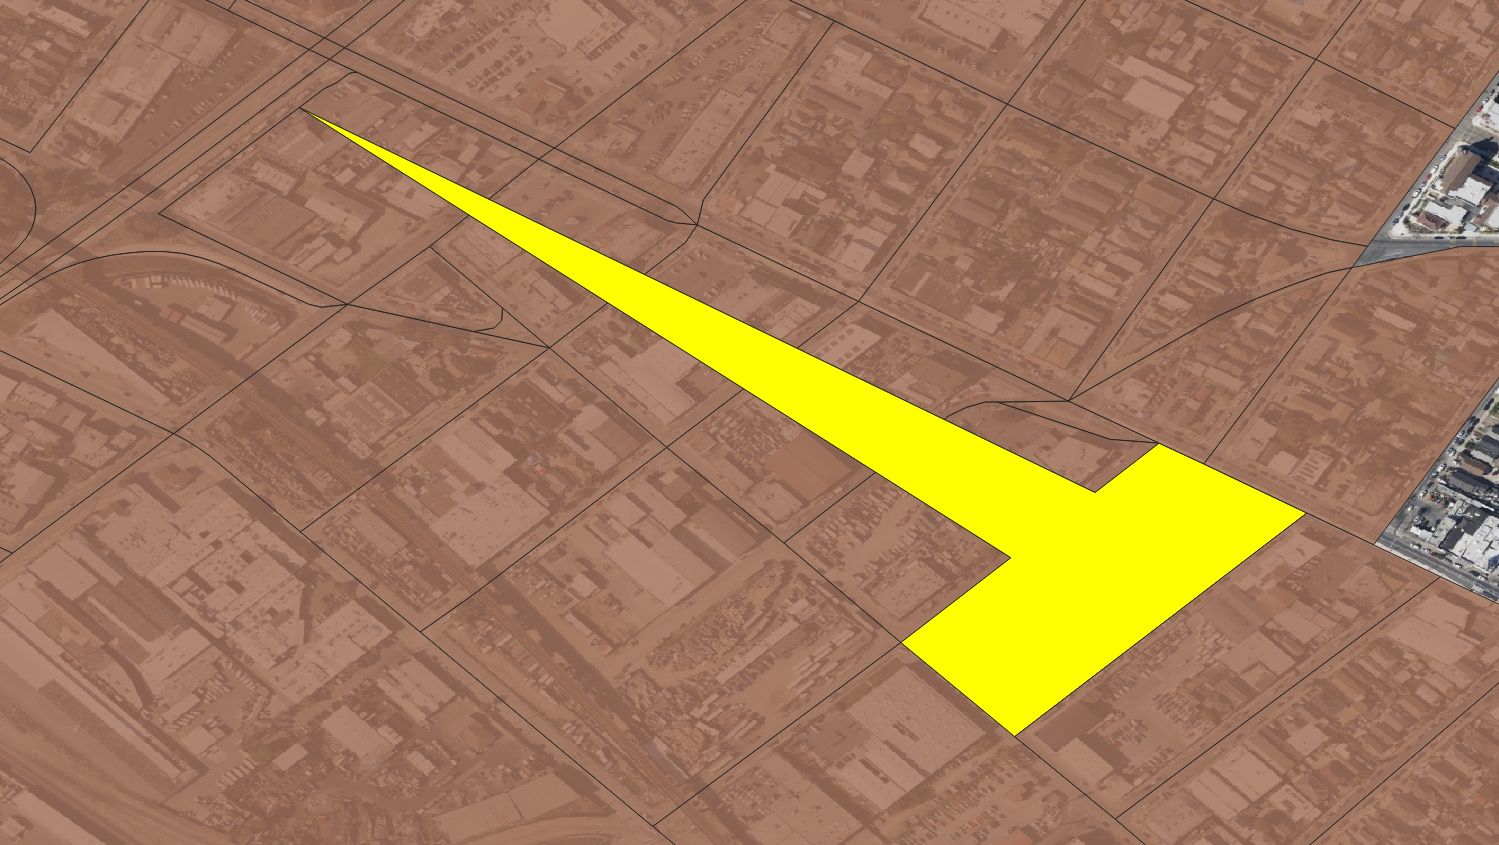
\includegraphics[width=0.8\textwidth]{figures/artifact02}
\end{frame}

\begin{frame}{Some invalids polygons...}
    \centering 
    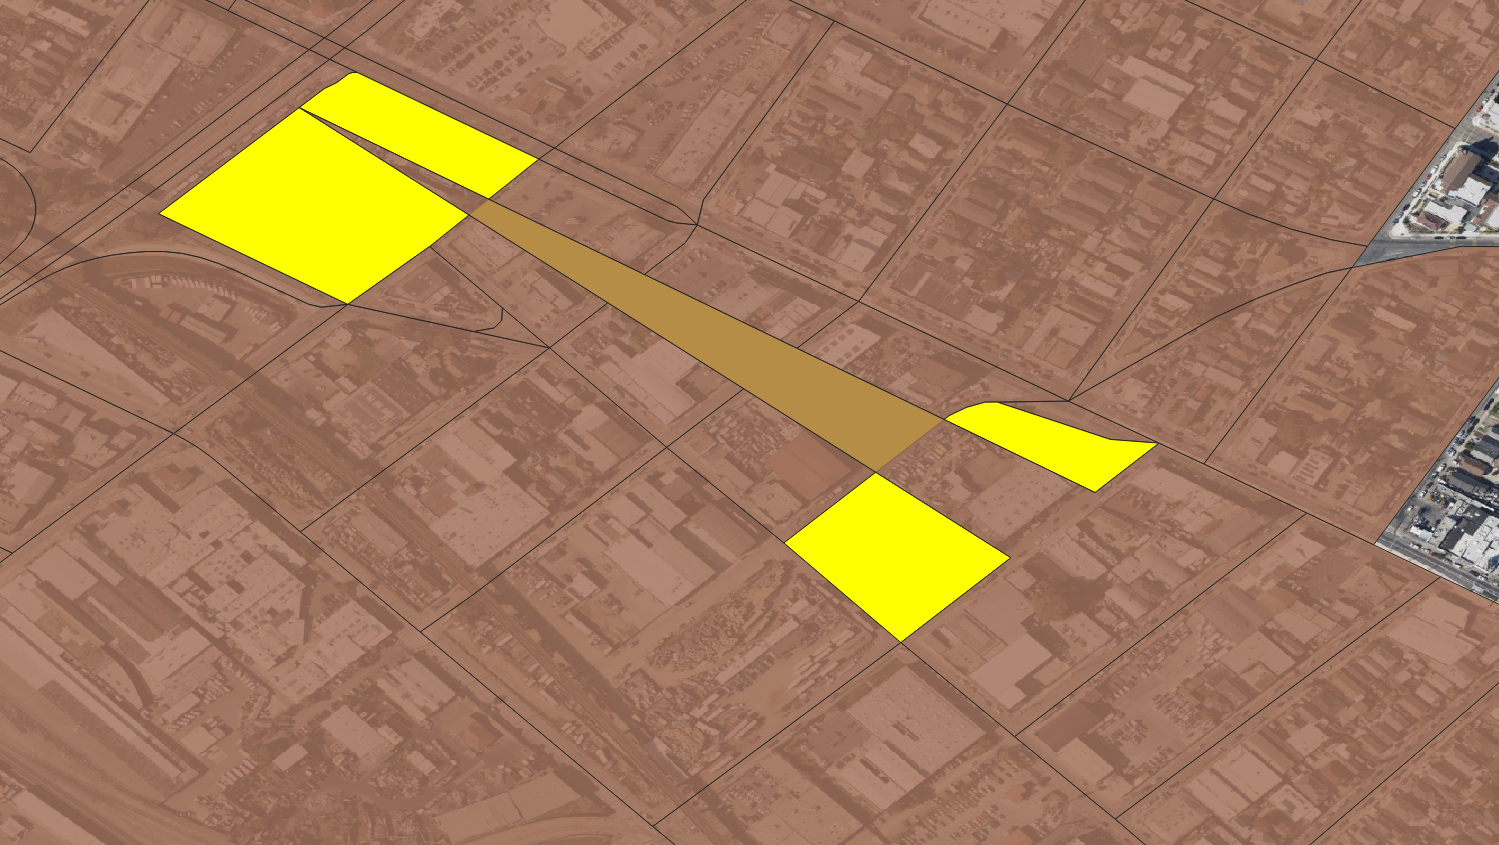
\includegraphics[width=0.8\textwidth]{figures/artifact01}
\end{frame}

\begin{frame}{Some invalids polygons...}
    \centering 
    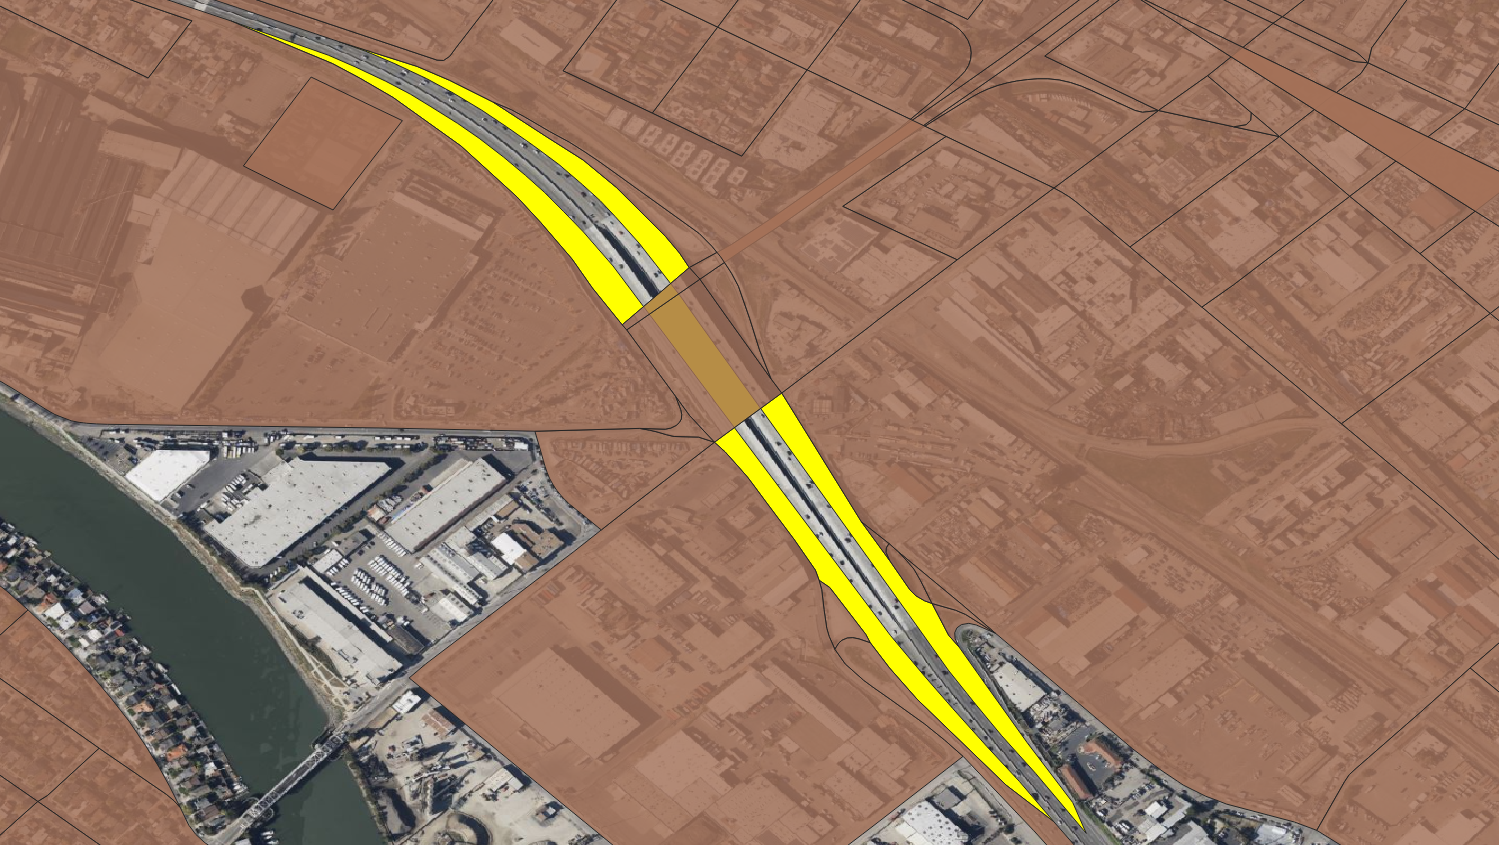
\includegraphics[width=0.8\textwidth]{figures/artifact03}
\end{frame}

\begin{frame}{What's next...}
  \begin{itemize}
    \item Define how to manage invalid polygons...
    \item Run additional tests with large datasets...
    \item Work on KD-tree partitioner (orphan holes?)...
  \end{itemize}
\end{frame}


\end{document}
